
\subsection{Powierzchnia Seiferta}
Zaczniemy od przyjrzenia się powierzchniom.
Niektóre stwierdzenia będziemy przyjmować bez dowodów, bo te są w~dobrych podręcznikach topologii albo analizy na rozmaitościach.

\begin{definition}
\index{powierzchnia}%
    Dwuwymiarową rozmaitość topologiczną bez brzegu $M \subseteq \R^n$ nazywamy powierzchnią.
\end{definition}

Rozmaitość to obiekt, który wygląda lokalnie jak przestrzeń euklidesowa: każdy jej punkt $x \in M$ posiada otwarte otoczenie homeomorficzne z~otwartą kulą.
Przykładami powierzchni są sfera, brzeg torusa albo hiperboloida jednopowłokowa.
Istnieje ogólniejsze pojęcie, to jest rozmaitość z~brzegiem: każdy jej punkt posiada otoczenie homeomorficzne z otwartym podzbiorem górnej półpłaszczyzny $\{x \in \C: \mathfrak {Im} \ge 0\}$.

%Zwartą powierzchnię bez brzegu nazywamy domkniętą.

Powierzchnię nazywamy orientowalną, jeśli nie istnieje na niej zamknięta krzywa, podczas pokonywania której odwraca się kierownica.
\index{powierzchnia!orientowalna}%
Orientowalne są dokładnie te powierzchnie, które nie zawierają w sobie kopii wstęgi Möbiusa.

\index{powierzchnia!Seiferta|(}%
Najważniejsze dla nas są powierzchnie Seiferta (opisane np. w \cite[s. 46-72]{kawauchi1996}, \cite[s. 19-21]{burde2014}).

\begin{definition}[powierzchnia Seiferta]
    Niech $L$ będzie splotem.
    Każdą spójną oraz orientowalną powierzchnię zanurzoną w przestrzeni $\R^3$, której brzegiem jest splot $L$, nazywamy powierzchnią Seiferta splotu $L$.
    % R^3, nie R^n: patrz Kawauchi, 47
\end{definition}

% TODO: potrzeba więcej przykładów w tej książce
% \begin{example}
% Powierzchnia Seiferta dla trójlistnika:
% \begin{center}
% \begin{tikzpicture}
% [scale=0.1]
%   \clip (-17,-15) rectangle (17,15);
%   \foreach \d in {0,180} {
%       \path[OBSZAR    ,rotate=\d] (-1.25,11.5)
%       .. controls (2,14) and (6,13.5) ..  (10,12)
%       .. controls (23,7) and (15,-20)  .. (3,-13)
%       -- (1.25, -11.5)
%       .. controls (4.5,-8) and (4.5,-4) .. (0,0)
%       .. controls (4,4) and (4.5,5.5) .. (-1.25,11.5);}
%   \path[TIKZ_ARCH] (0,10) .. controls (10,0) and (-10,0) .. (0,-10);
%   \foreach \d in {0,180} {
%   \path[TIKZ_ARCH, rotate=\d] (-1.5,1.5) .. controls (-6,6) and (-3,17) .. (10,12)
%   .. controls (23,7) and (15,-20)  .. (3,-13);}
% \end{tikzpicture}
% \end{center}
% \end{example}

% TODO: dorysować to, co widać po standardowym...
Nie każde uszachowienie diagramu węzła prowadzi do powierzchni Seiferta: widać to po standardowym diagramie trójlistnika.
Pomimo to...

\begin{proposition}
\label{prp:seifert_exists}%
    Każdy splot posiada powierzchnię Seiferta.
\end{proposition}

Powyższe stwierdzenie uzasadnili Pontriagin oraz Frankl w~1930 roku, my jednak podamy przyjemny i~konstruktywny dowód podany przez Seiferta \cite{seifert1935} cztery lata później.
\index[persons]{Seifert, Herbert}%
% TODO: Frankl, F.; Pontrjagin, L. (1930). "Ein Knotensatz mit Anwendung auf die Dimensionstheorie". Math. Annalen (in German). 102 (1): 785–789. doi:10.1007/BF01782377.
(Piszą o tym na początku swojej monografii Burde, Zieschang, Heusener \cite[s. 19]{burde2014}).

\begin{proof}
\index{algorytm!Seiferta|(}%
    Wybierzmy diagram $D$ dla splotu oraz orientację,
    a~następnie wyprostujmy wszystkie skrzyżowania zgodnie z~ich orientacją:
\begin{comment}
    \[
        \LargeMinusCrossingArrows, \LargePlusCrossingArrows \longrightarrow \LargeThikkJustSmoothing
    \]
\end{comment}

    Otrzymany diagram składa się teraz z~pewnej liczby zamkniętych krzywych,
    zwanych okręgami Seiferta, które wypełniamy do dysków.
    Tam, gdzie jeden okrąg leżał wewnątrz drugiego, podnosimy wewnętrzny nad zewnętrzny.
    Przy każdym skrzyżowaniu pierwotnego diagramu doklejamy skręcony pasek do obydwu dysków.

    \begin{figure}[H]
        \centering
        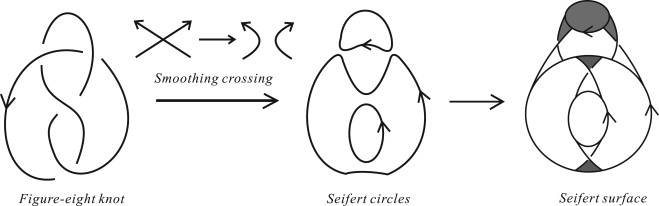
\includegraphics[width=0.75\textwidth]{../data/seifert-algorithm.jpg}
        \caption[Smthing]{Kolejne kroki algorytmu Seiferta}
    \end{figure}

    Pozostało wskazać orientację dla tak otrzymanej powierzchnii.
    Przypisujemy znak $+$ górnej stronie dysków, których brzeg jest zorientowany dodatnio (oraz dolnej stronie dysków, których brzeg jest zorientowany ujemnie).
\index{algorytm!Seiferta|)}%
\end{proof}

Powierzchnia Seiferta jest wrażliwa na orientację ogniw splotu: odwrócenie niektórych, ale nie wszystkich, często prowadzi do innej powierzchni.
Na przykład sygnatura splotu L4a1 może wynosić, w zależności od orientacji ogniw względem siebie, $1$ lub $-3$.

\index{powierzchnia!Seiferta|)}%

% Węzeł jest rozwłókniony dokładnie wtedy, gdy stanowi grzbiet pewnego 'open book decomposition' $S^3$.

